
\documentclass[border=10pt]{standalone}
\usepackage{pgfplots}
\pgfplotsset{compat=1.18}
\begin{document}
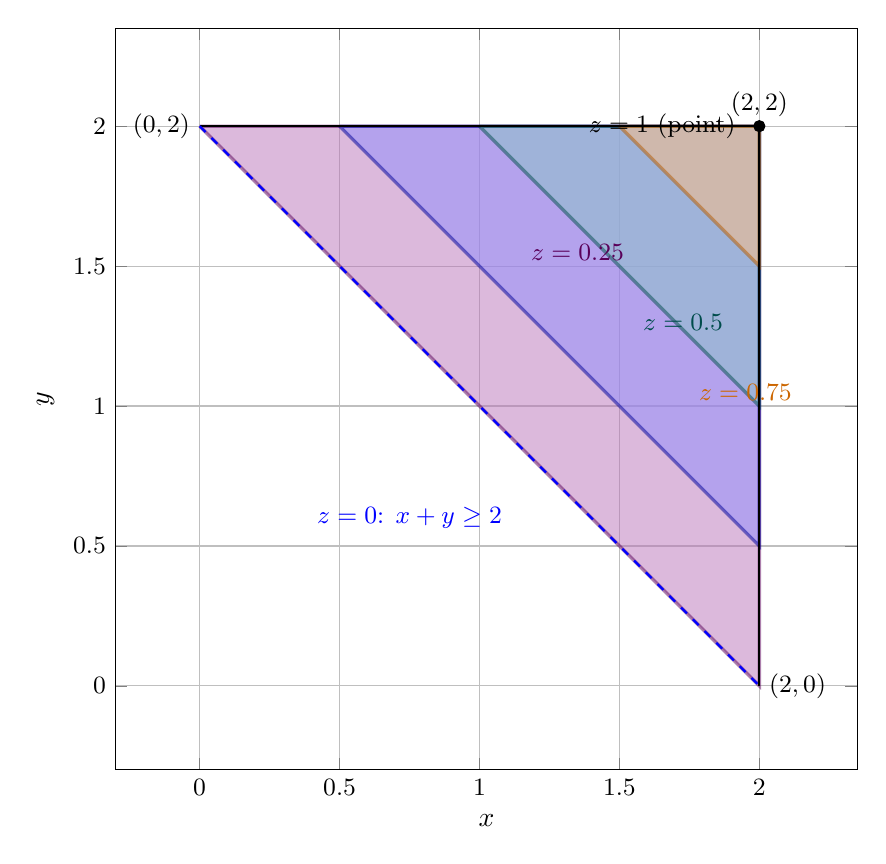
\begin{tikzpicture}
\begin{axis}[
    xlabel={$x$}, ylabel={$y$},
    xmin=-0.3, xmax=2.35, ymin=-0.3, ymax=2.35,
    width=11cm, height=11cm,
    axis equal image,
    grid=both,
    tick label style={font=\small},
]
\addplot[fill=violet!55,opacity=0.5,draw=violet!70!black,very thick] coordinates {(0,2) (2,2) (2,0) (0,2)};
\addplot[fill=blue!45,opacity=0.5,draw=blue!60!black,very thick]    coordinates {(0.5,2) (2,2) (2,0.5) (0.5,2)};
\addplot[fill=teal!45,opacity=0.5,draw=teal!60!black,very thick]    coordinates {(1,2) (2,2) (2,1) (1,2)};
\addplot[fill=orange!50,opacity=0.5,draw=orange!70!black,very thick] coordinates {(1.5,2) (2,2) (2,1.5) (1.5,2)};
\addplot[only marks,mark=*,mark size=2pt,black] coordinates {(2,2)};
% guide lines
\addplot[black,thick] coordinates {(0,2) (2,2)};
\addplot[black,thick] coordinates {(2,0) (2,2)};
\addplot[blue,dashed,thick] coordinates {(0,2) (2,0)};

\node[anchor=south,font=\small] at (axis cs:2,2) {$(2,2)$};
\node[anchor=east,font=\small]  at (axis cs:0,2) {$(0,2)$};
\node[anchor=west,font=\small]  at (axis cs:2,0) {$(2,0)$};
\node[blue,font=\small] at (axis cs:0.75,0.6) {$z=0$: $x+y\ge 2$};
\node[violet!70!black,font=\small,anchor=west] at (axis cs:1.15,1.55) {$z=0.25$};
\node[teal!60!black,font=\small,anchor=west] at (axis cs:1.55,1.30) {$z=0.5$};
\node[orange!80!black,font=\small,anchor=west] at (axis cs:1.75,1.05) {$z=0.75$};
\node[black,font=\small,anchor=east] at (axis cs:1.95,2.0) {$z=1$ (point)};
\end{axis}
\end{tikzpicture}
\end{document}
